\subsection{Fragmented orbital matches and three further valence tests}
The fixed $\eta=0.60$ candidate is next applied to cyclopropene,
cyclopentadiene, and pyrrole. All three predictions are archived before
extracting their numerical QUEST references. Their errors are initially
$+0.054$, $-0.013$, and $+2.369$ eV. Historical exposure of some of these
molecules prevents a strictly blind claim. Pyrrole's discrepancy exposes
a reference-construction limitation: its native virtual orbitals have
substantial weight distributed over several full-DFT virtual orbitals,
so no individual match meets the existing 0.7 amplitude criterion.
The original fallback therefore omits both the qualified Q level and the
complement relaxation for these orbitals.

We amend this rule for \emph{every} unresolved occupied or virtual orbital,
without a molecule or state-family branch. Within the same occupation
sector, full-DFT poles are ordered by native spectral weight $w_{ki}$.
The smallest block $\mathcal B_i$ satisfying
$\sum_{k\in\mathcal B_i}w_{ki}\geq0.7^2$ supplies the normalized centroid
\begin{equation}
 \mu_i=\frac{\sum_{k\in\mathcal B_i}w_{ki}\epsilon_k}
 {\sum_{k\in\mathcal B_i}w_{ki}} .
\end{equation}
This centroid supplies the Q level with the original occupied-centroid
alignment. Its difference from the Rayleigh energy of the original
native image supplies the unresolved F relaxation. Individually qualified
poles retain their preceding treatment. We then rebuild the explicit
bath screening on the corrected native orbitals. The 50/50 average,
$\lambda=0.9$, $\eta=0.60$, configuration rule and zero energy offset remain
fixed. This is a diagonal spectral-centroid approximation, not an exact
elimination of a broad or frequency-dependent environment. The reference
preparer reads no excitation labels, but the amendment was developed after
pyrrole scoring: the resulting ledger is an exposed development assessment.

Pyrrole then gives 6.302 eV against 6.247 eV. Applying the identical rule
to all 26 states in 24 molecules gives MAE 0.198 eV and maximum error
0.446 eV. The twelve $\pi\pi^*$ states give 0.216 eV MAE; the fourteen
$n\pi^*$ states give 0.183 eV. All individual errors are below 0.5 eV.
Matched TDA on the corrected native GFN2 orbitals gives 0.789 eV MAE
overall, 1.514 eV for $\pi\pi^*$ and 0.168 eV for $n\pi^*$: the OO gain
is concentrated in the $\pi\pi^*$ family, while TDA has the smaller mean
$n\pi^*$ error. Neither comparison is a calibrated sTDA-xTB benchmark.
Every prepared state passes fresh-process spin and restart checks with no
DFT import, new SCC call or TDA solve. Ethylene's updated full analytic
Hessian takes 10.68 s; scalar-energy Richardson checks give errors below
$9.92\times10^{-12}$ Ha/bohr and $2.46\times10^{-8}$ Ha/bohr$^2$.
These remain derivatives of a frozen anchored model.

\begin{figure}[!htbp]\centering
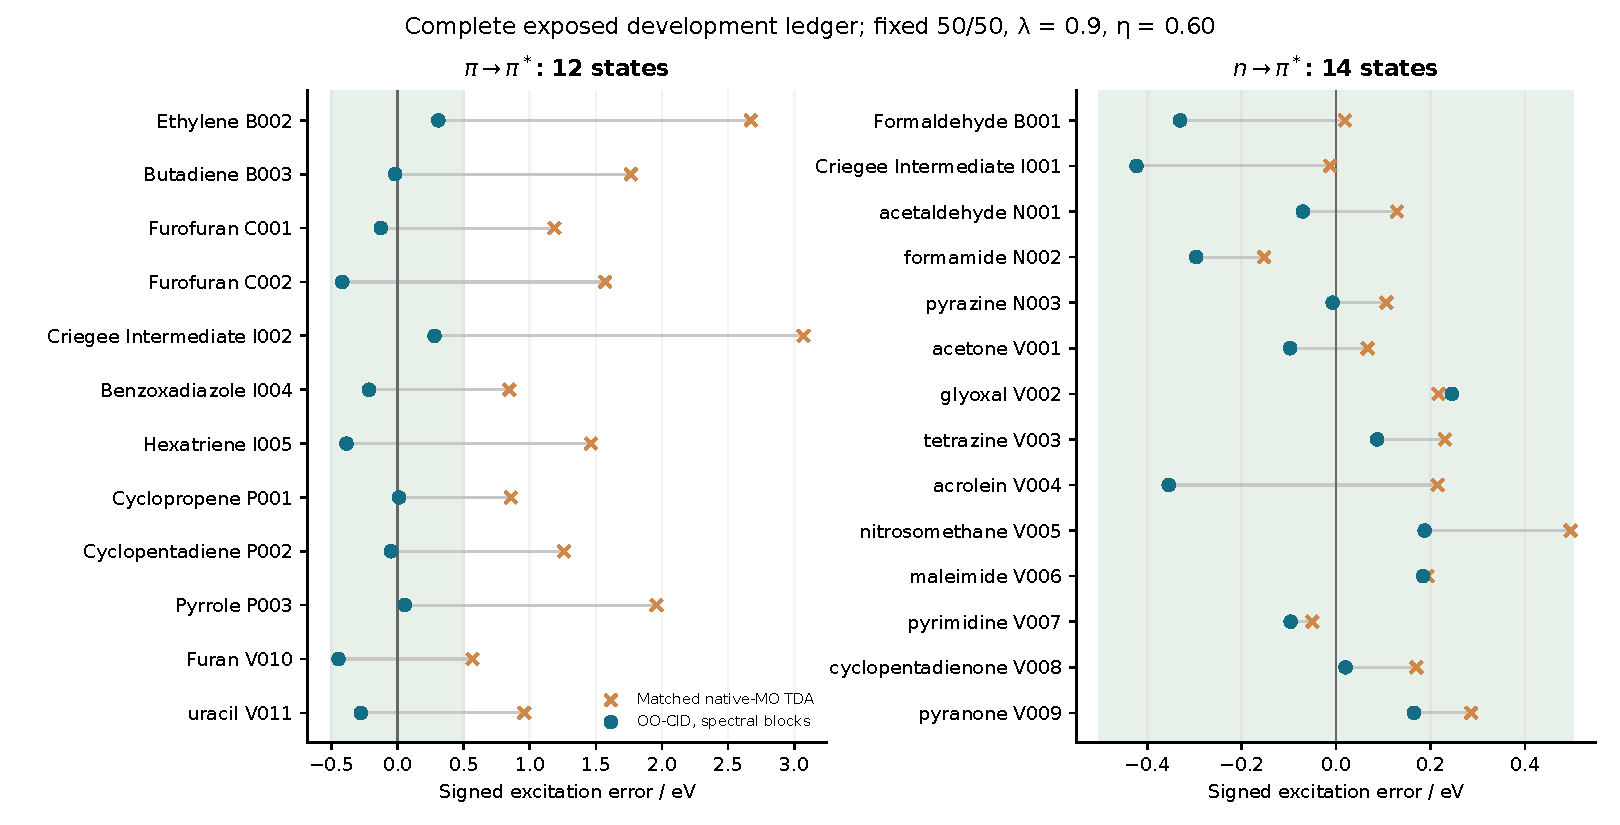
\includegraphics[width=\linewidth]{figures/spectral_block_validation.pdf}
\caption{All 26 exposed development states after the generic spectral-block
reference amendment. Points compare OO-CID with freshly calculated TDA on
the same corrected native orbitals. The shaded interval is $\pm0.5$ eV.
The two panels use different horizontal scales. Neither the bath efficiency
nor the F/Q weights are retuned for the three added molecules.}
\label{fig:spectralblocks}
\end{figure}

\subsection{Larger pigment structures: preparation scope}
We select all-trans $\beta$-carotene and chlorophyllide a as larger
chromophore tests. Chlorophyllide a retains Mg and the conjugated
substituents while removing the phytyl chain. Figure~\ref{fig:pigmentstructures}
shows the actual source structures, rather than schematic molecular art.
Native ground checkpoints contain 216 and 219 orbitals, respectively.
The chlorophyllide reconstruction explicitly includes Mg d functions.
Raw Gaussian-overlap discrepancies and subsequent numerical metric
reconciliation are archived separately; agreement after reconciliation is
$2.5\times10^{-13}$ or better. The one-time PBE0/CAM-B3LYP reference
preparation uses checkpointed RI-JK calculations on the verified Mac Studio.
No pigment excitation energy, excited minimum or Hessian is claimed here,
and these molecules are excluded from the 26-state accuracy pool.
Nonplanar configuration selection, the distinction between dark and bright
carotenoid states, and mixing of chlorophyll Q-band targets require explicit
qualification before extending the model's demonstrated scope.

\begin{figure}[p]\centering
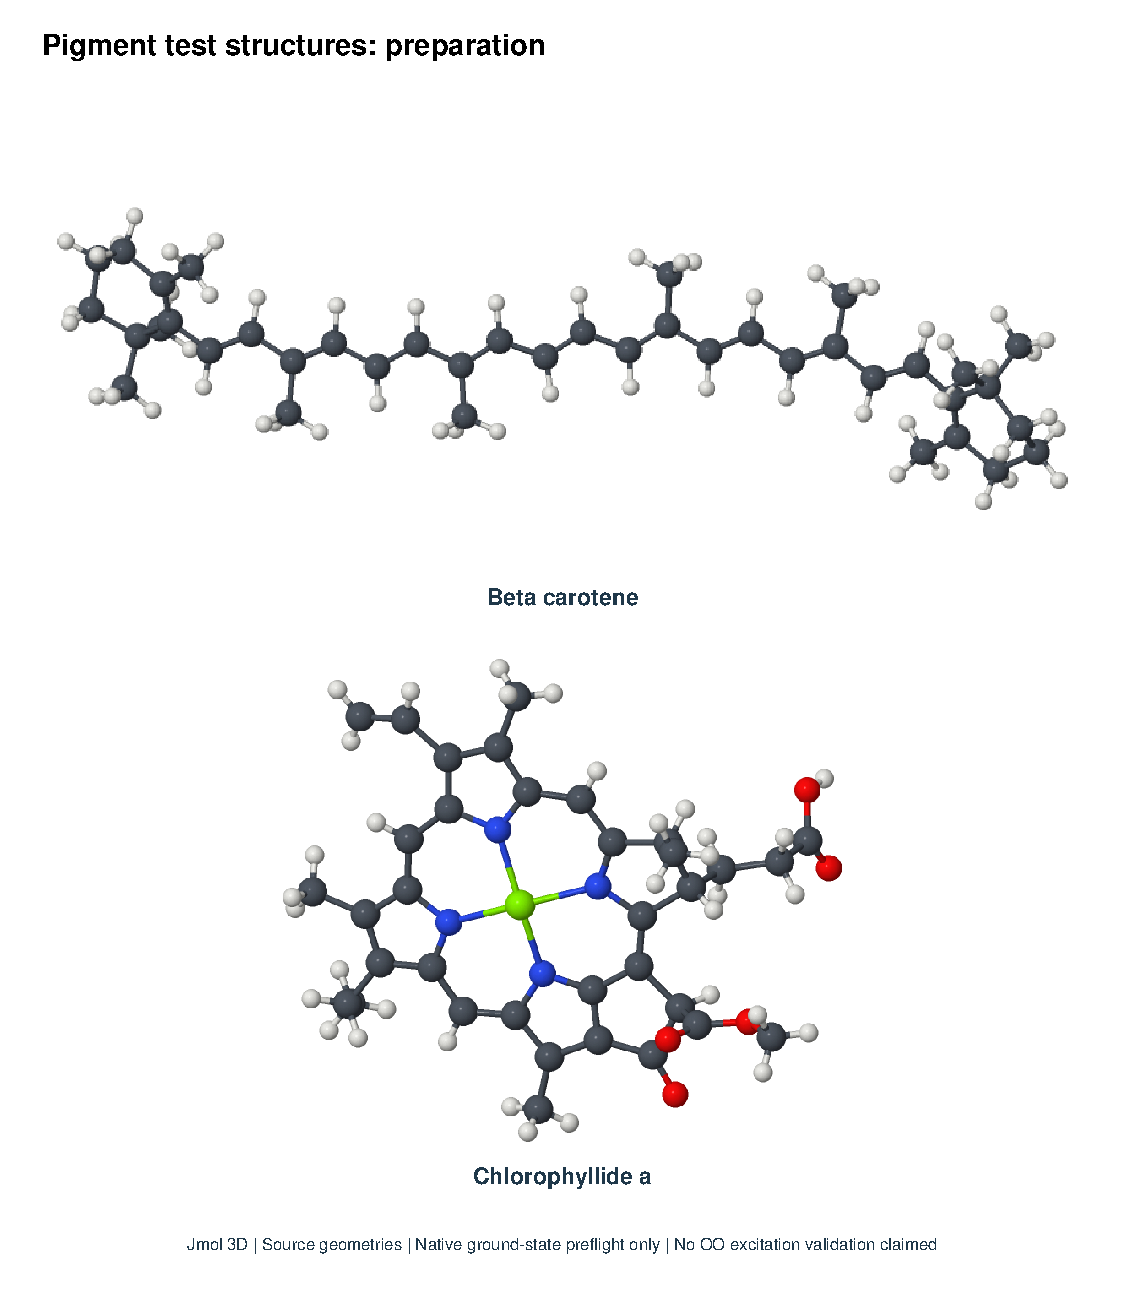
\includegraphics[width=.92\linewidth,height=.80\textheight,keepaspectratio]{figures/pigment_test_structures_jmol.pdf}
\caption{Jmol renderings of the larger starting structures: all-trans
$\beta$-carotene (96 atoms; PubChem CID 5280489) and chlorophyllide a
(79 atoms; RCSB ligand A1JWG). These primary-source geometries are used
for preparation and are not optimized excited-state structures or
validated additions to the accuracy ledger.}
\label{fig:pigmentstructures}
\end{figure}
